%27/10 - Paco Jurado
\chapter{Parseo de constituyentes}
\section{Lenguaje formal y constituyentes}
Hay dos formas de parseos: el parseo de constituyentes (forma de árbol) y análisis de dependencias (saltos a partir del verbo raíz para sacar las relaciones). 

\begin{figure}[h]
\centering
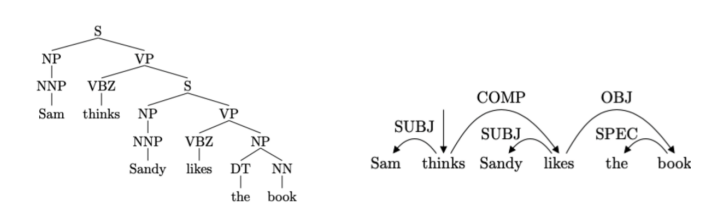
\includegraphics[width = \textwidth]{figs/parseo.png}
\end{figure}

La constitución sintáctica es la idea de que los grupos de palabras pueden comportarse como unidades únicas: constituyentes. Parte del desarrollo de una gramática implica crear un inventario de los constituyentes del idioma.

\section{Gramática libre de contexto}
La gramática libre de contexto o gramáticas de estructura sintáctica son el sistema formal más utilizado para modelar la estructura constituyente del inglés y otras lenguas naturales.

Un CFG consiste en un conjunto de reglas o producciones, cada una de las cuales expresa las formas en que los símbolos del lenguaje pueden agruparse y ordenarse, y un léxico de palabras y símbolos. 

El lenguaje formal definido por una CFG es el conjunto de cadenas que se pueden derivar del símbolo inicial designado. Cada gramática debe tener un símbolo inicial designado, que a menudo se denomina S. Dado que las gramáticas libres de contexto se utilizan a menudo para definir oraciones, S se interpreta normalmente como el nodo «oración», y el conjunto de cadenas que se pueden derivar de S es el conjunto de oraciones en una versión simplificada del inglés. 

Tenemos el lexicón con opciones de nombres, verbos, adjetivos, etc. Esos son los símbolos terminales. También hay reglas de producción: la frase está compuesta por nombre y predicado. El nombre puede ser un pronombre, nombre propio o determinante nominal. El predicado verbal puede ser verbo, verbo con nombre, verbo con nombre con preprosición, etc. Dado así un árbol construido con el análisis, se busca identificar si se ha podido generar con la gramática y los símbolos terminales. En esto consiste el análisis de la estructura de la oración. 

Las gramáticas libres de contexto vienen definidos por los signos no terminales.

\begin{figure}[h]
\centering
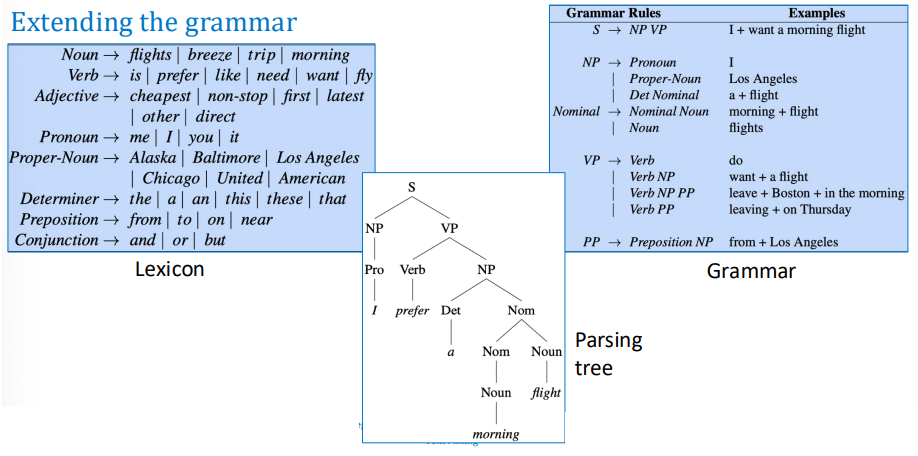
\includegraphics[width = 0.8\textwidth]{figs/grammar.png}
\end{figure}

\section{Parseo libre de contexto}
El parseo es la tarea de determinar si una cadena puede derivarse de una gramática libre de contexto dada y, en caso afirmativo, cómo. La estructura del análisis sintáctico puede responder a preguntas básicas del tipo «quién hizo qué a quién». Es útil para diversas tareas posteriores, como el análisis semántico, la traducción automática y la extracción de información.

Solo es posible realizar una búsqueda exhaustiva del espacio de análisis sintácticos recurriendo a supuestos de localidad. Estos permiten realizar búsquedas eficientes reutilizando subestructuras compartidas con programación dinámica.

El \textbf{algoritmo CKY} tiene un enfoque ascendente para el análisis sintáctico en una gramática libre de contexto. Comprueba de forma eficiente si una cadena pertenece a un lenguaje, sin enumerar todos los análisis sintácticos posibles. El algoritmo primero forma pequeños constituyentes y, a continuación, intenta fusionarlos en constituyentes más grandes.

El algoritmo va realizando las agrupaciones partiendo de los símbolos terminales de la oración (lo que estamos leyendo y recibiendo) y agrupa para ir creando los constituyentes. Para que funcione bien, las gramáticas no pueden estar escritas de cualquier modo; tienen que estar escritas en CNF, un símbolo no terminal que lleva a dos símbolos no terminales o a un símbolo terminal. Esto permite así agrupar de dos en dos.

\begin{figure}[h]
\centering
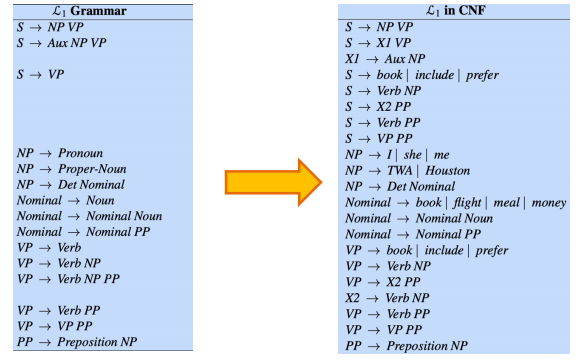
\includegraphics[width = 0.8\textwidth]{figs/cnf.png}
\end{figure}

\section{Gramáticas libres de contexto probabilísticas}
Se aplica la estadísitca para anotar las oraciones con treebanks y aprender modelos probabilísticos que infieran las reglas de producción. 

Se pueden utilizar gramáticas suficientemente robustas, compuestas por reglas gramaticales libres de contexto, para asignar un árbol sintáctico a cualquier oración. Esto significa que es posible construir un corpus en el que cada oración de la colección se empareje con un árbol sintáctico correspondiente. Este tipo de corpus con anotaciones sintácticas se denomina banco de árboles. Los bancos de árboles desempeñan un papel importante en el análisis sintáctico, así como en las investigaciones lingüísticas de los fenómenos sintácticos.

\begin{figure}[h]
\centering
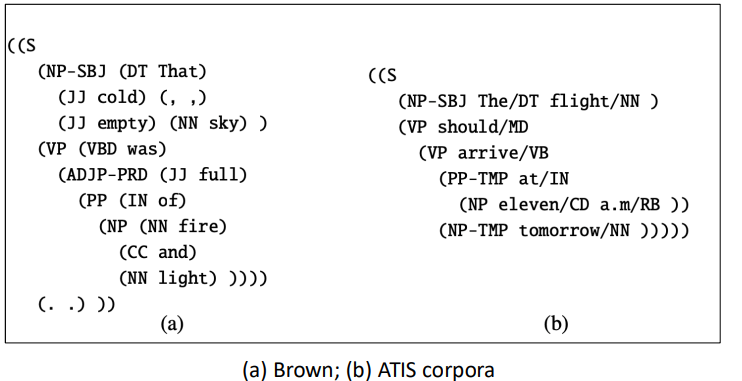
\includegraphics[width = 0.6\textwidth]{figs/treebank.png}
\end{figure}

Tenemos símbolos terminales (palabras), no terminales (constituyentes, PoS tag), reglas de producción, símbolo inicial y reglas de probabilidad. 

En las gramáticas libres de contexto, se agrupan dos a dos las reglas estrictas. Ahora, se hace lo mismo teniendo en cuenta la probabilidad de las reglas de producción. En otras palabras, se añade probabilidad al algoritmo CKY con argmax. 

\section{Evaluar parsers}
Para comparar los distintos enfoques de análisis sintáctico, necesitamos medir su rendimiento. Supongamos que tenemos un conjunto de análisis sintácticos de referencia (ground truth) etiquetados manualmente; por lo general, estos análisis sintácticos de referencia se extraen de un banco de árboles sintácticos como el Penn Treebank. Una solución sencilla sería la precisión por frase: el analizador se puntúa según la proporción de frases en las que el sistema y los análisis de referencia coinciden exactamente. La \textbf{métrica PARSEVAL} mide en qué medida los constituyentes del árbol de análisis hipotético se parecen a los constituyentes del análisis de referencia.

También se pueden utilizar recall y precisión. Un constituyente en un análisis hipotético Ch de una oración s se etiqueta como correcto si hay un constituyente en el análisis de referencia Cr con el mismo punto de inicio, punto final y símbolo no terminal. 

$$\text{labeled recall} = \frac{\text{\# of correct constituents in hypothesis parse of s}}{\text{\# of correct constituents in reference parse of s}}$$

$$\text{labeled precision} = \frac{\text{\# of correct constituents in hypothesis parse of s}}{\text{\# of total constituents in reference parse of s}}$$

La alternativa son las agrupaciones: El número de constituyentes para los que el análisis de referencia tiene un corchete como ((A B) C), pero el análisis hipotético tiene un corchete como (A (B C)).